\documentclass[tikz]{standalone}

\usepackage{import}
\usepackage{tikz}
\usepackage{amsmath}

\newcommand{\radius}{4}
\newcommand{\circlesize}{5.50}
\newcommand{\circleopacity}{.33}

\newcommand{\thetaone}{0}
\newcommand{\thetatwo}{1.570796}
\newcommand{\thetathree}{3.141593}
\newcommand{\thetafour}{4.712389}

\newcommand{\pone}{(\fpeval{\radius*cos(\thetaone)},\fpeval{\radius*sin(\thetaone)})}
\newcommand{\ptwo}{(\fpeval{\radius*cos(\thetatwo)},\fpeval{\radius*sin(\thetatwo)})}
\newcommand{\pthree}{(\fpeval{\radius*cos(\thetathree)},\fpeval{\radius*sin(\thetathree)})}
\newcommand{\pfour}{(\fpeval{\radius*cos(\thetafour)},\fpeval{\radius*sin(\thetafour)})}

\newcommand{\VennTextScale}{2}
\begin{document}
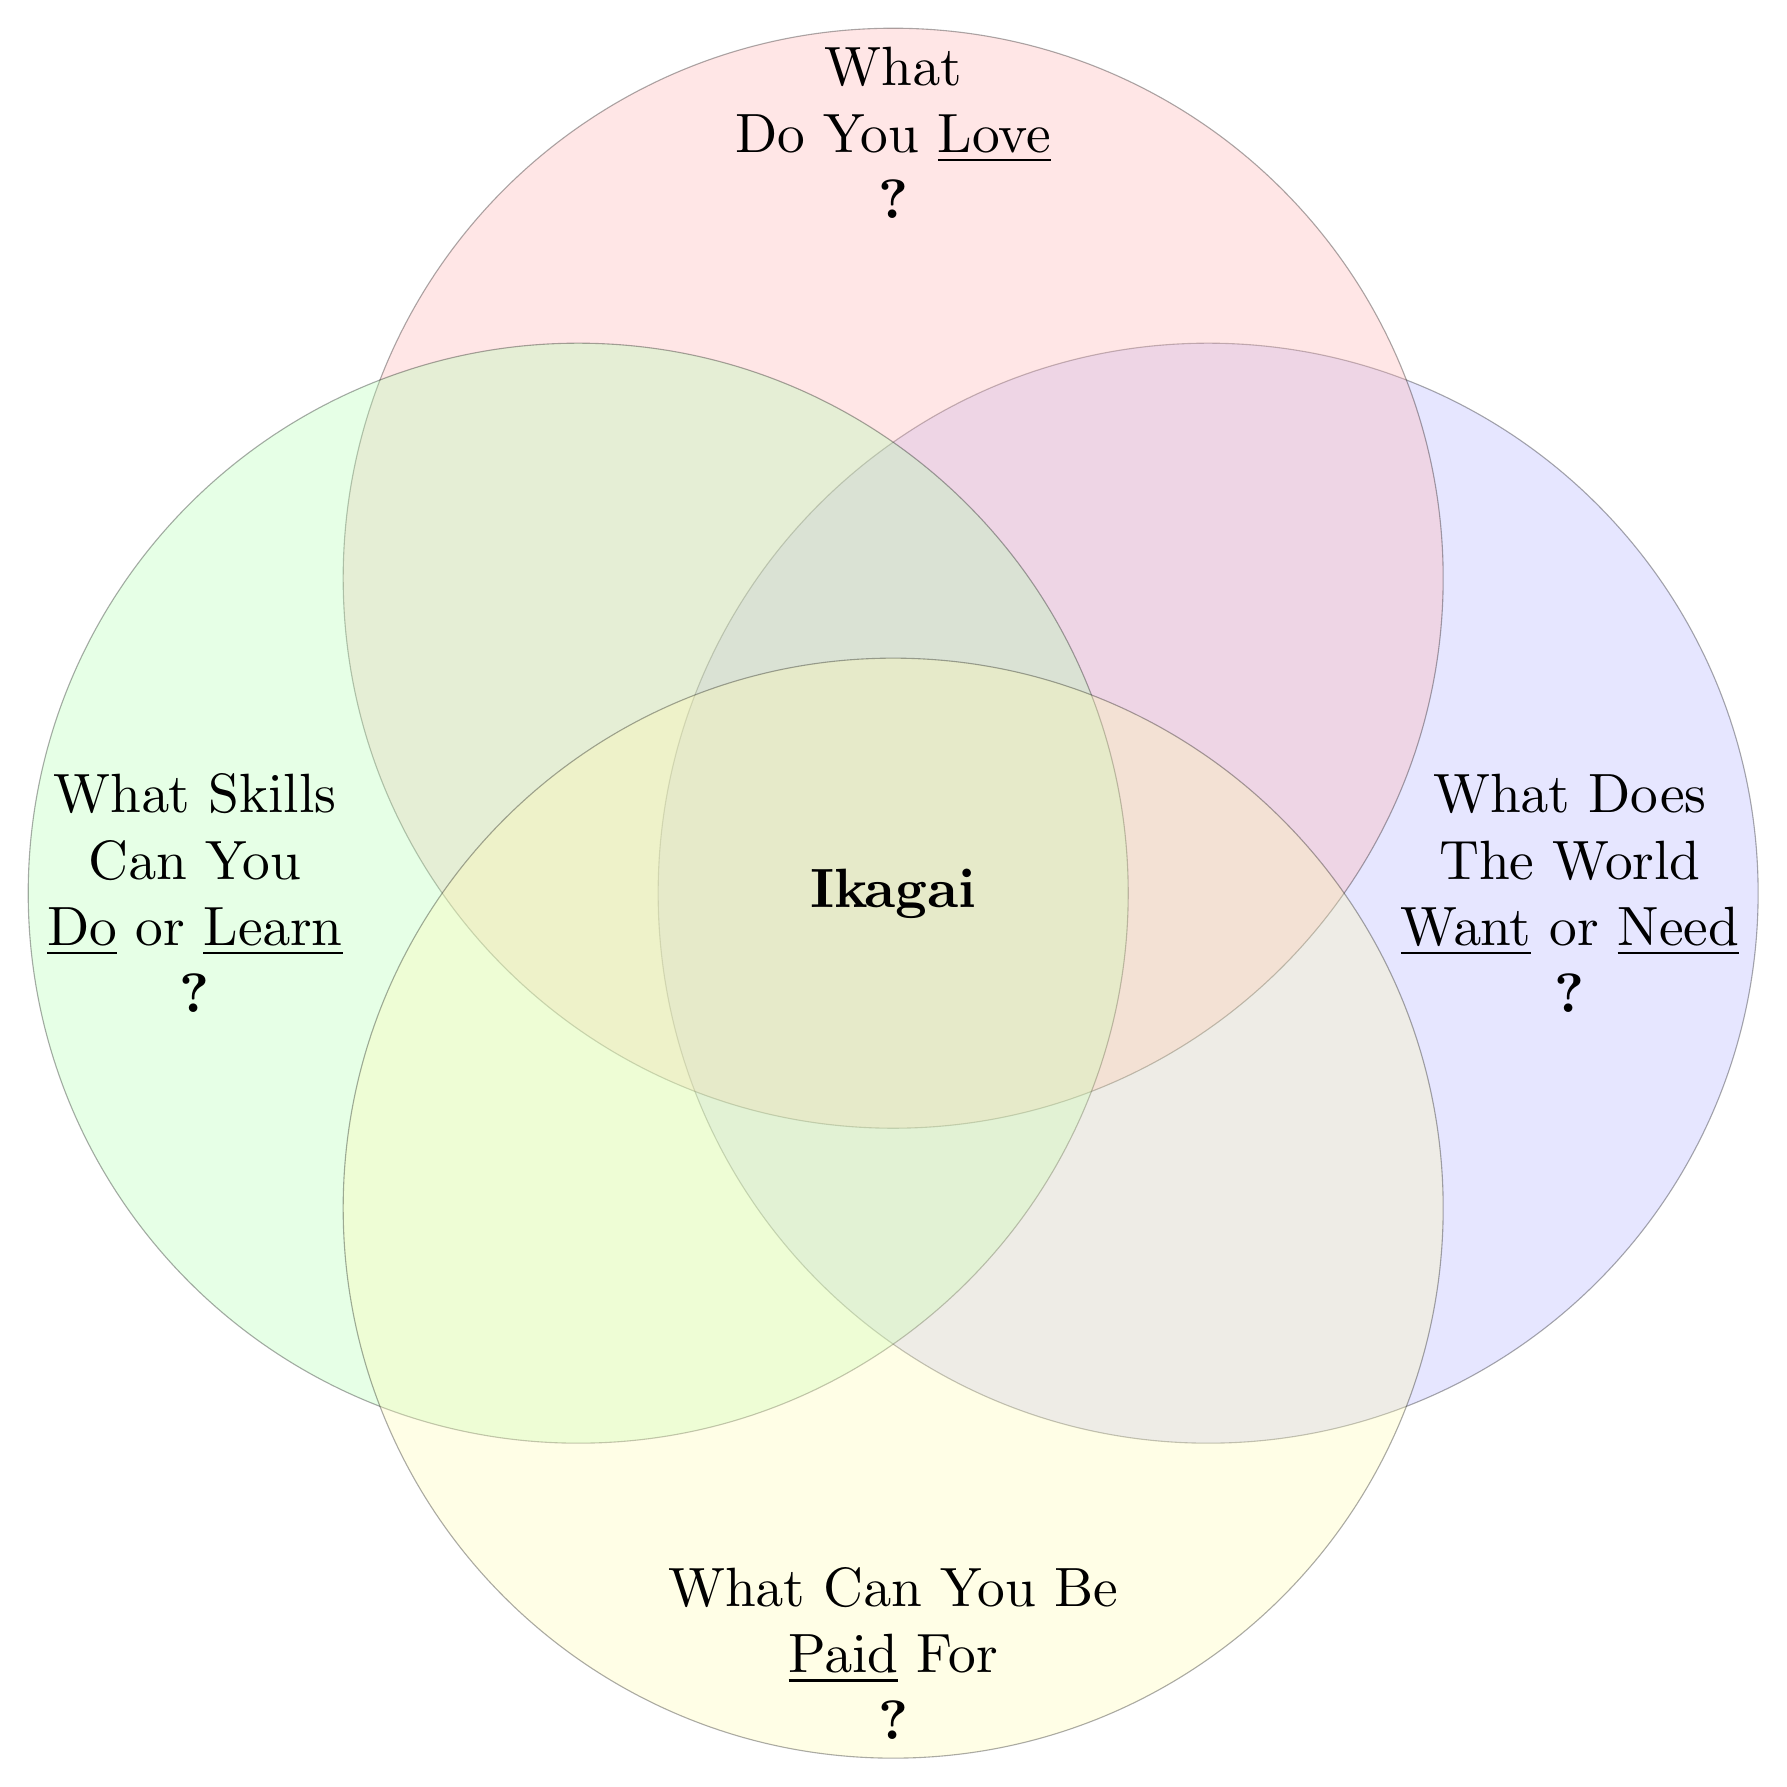
\begin{tikzpicture}

% Venn Diagram Nodes
\node (EC) [draw=black,circle,fill=blue!30,opacity=\circleopacity, minimum size=\circlesize in ] at  \pone  {};
\node (NC) [draw=black,circle,fill=red!30,opacity=\circleopacity, minimum size=\circlesize in ]  at \ptwo  {};
\node (WC) [draw=black,circle,fill=green!30,opacity=\circleopacity, minimum size=\circlesize in ]  at \pthree  {};
\node (SC) [draw=black,circle,fill=yellow!30,opacity=\circleopacity, minimum size=\circlesize in] at  \pfour  {};

% Label the nodes
\node[anchor=east,align=center,scale=\VennTextScale] at (EC.east) {What Does \\ The World \\\underline{Want} or \underline{Need}\\\textbf{?}};
\node[anchor=west,align=center,scale=\VennTextScale] at (WC.west) {What Skills \\ Can You \\\underline{Do} or \underline{Learn}\\\textbf{?}};
\node[anchor=north,align=center,scale=\VennTextScale] at (NC.north) {What  \\ Do You \underline{Love} \\\textbf{?}};
\node[anchor=south,align=center,scale=\VennTextScale] at (SC.south) {What Can You Be \\ \underline{Paid} For\\\textbf{?}};

%Background node
\node[align=center,scale=\VennTextScale] at (0,0) {\textbf{Ikagai}};


\end{tikzpicture}
\end{document}
